\newpage
\section{Independent Q-Learning}\label{sec:IQL}
Q-Learning is an off-policy temporal difference control algorithm. Temporal difference methods can learn directly from raw experience without a model of the environment's dynamics. Furthermore, it updates estimates based in part on other learned estimates, without waiting for a final outcome \cite[pp. 133]{RL1}. 

While the distinguishing feature of on-policy methods is that they estimate the value of a policy while using it for control, these two functions are separated in off-policy methods. The behavior policy, used to generate behavior, and the estimation policy, that is evaluated and improved, may in fact be unrelated. This separation is an advantage because the estimation policy may be deterministic (e.g., greedy), while the behavior policy can continue to sample all possible actions \cite[pp. 126]{RL1}. Its simplest form, \emph{one-step Q-learning}, is defined by \cite[pp. 148]{RL1}:
\begin{align*}
Q(s_t,a_t) & \leftarrow Q(s_t,a_t) + \alpha \left[ r_{t+1} + \gamma \displaystyle\max_a Q(s_{t+1},a) - Q(s_t,a_t) \right]
\end{align*}
When using Q-Learning in a multi-agent setting independently for each agent, the method is called Independent Q-Learning (IQL). In IQL, for a single agent, all the other agents are modeled as part of the environment. While Q-Learning is guaranteed to converge, Independent Q-Learning is not guaranteed to converge. This is because the premise of the convergence porperty of Q-Learning is that the environment be stationary. This will not be the case in a multiagent setting in which agents are learning concurrently, since the agents base their policy upon the movements of the other agents which are also learning. That is, the other agents don't act deterministically but are modeled as such. Independent Q-Learning can thus not be justified theoretically \cite[pp. 57]{vlassis}.

\subsection{Implementation}
For this assignment, we implemented Independent Q-learning and used it independently for all our agents, the predators and the prey. The agents learn concurrently (i.e. all agents do a move, then all update their estimated values), not sequentially (i.e. after one agent does a move, all other agents update their estimated values). When any two predators bump into each other, the prey wins (reward of $10$) and the predators all lose (reward of $-10$). When a predator catches the prey, the prey loses and all predators win.

 Each agent will have its own state representation and learning and will view the other agents as part of the environment. We used $\epsilon$-greedy action selection, which behaves greedily most of the time, but with probability $\epsilon$, instead select an action at random, uniformly, independently of the action-value estimates \cite[pp. 28]{RL1}. In this case, we used $\epsilon = 0.1$. We initiated the values of each Q-learning table optimistically with a value of 15 for all cells for the tables.

\subsubsection{State space} \label{sec:stateSpaceIQL}
The state space is of crucial importance to Independent Q-Learning, because it grows exponentially with the number of agents. In the experiments described in the previous report, were we had just one prey and one predator, we initially used a state space that was an intuitive, yet cumbersome representation. We then changed the state space representation to a more efficient one in the second assignment, referred to as the `efficient' state space, which led to a reduction of 697 times less states, resulting in just 21 different states. See Section \ref{sec:stateSpaceIntro} for details.

The default amount of states for this assignment would be $121^{p+1}$ for each agent, where p equals the number of predators. By using the efficient state space this has been reduced to $21\cdot 121^{p-1}$ because the prey's position is fixed in the state space representation and the predator to which this state space belongs moves along those $21$ states, the rest is used to determine in which state the predator currently resides. In this assignment however the prey also learns, so to make use of our state space representation, a single predator will be used as reference point every time so that the predator is fixed at the position $(0, 0)$ in our state space and the prey would be moving around the $21$ states just like a predator. 

The reduction is increased further by pointing to the same state for each combination of current positions of the other predators, though this is only effective for more than two predators. A simple example would be a case three predators and a prey, the current predator ($p_1$) which has to find his current state would take the position of the first other predator ($p_2$) and then the position of the second other predator ($p_3$) to locate his state in the state space. In this case it shouldn't matter which position, $p_2$ or $p_3$, would be looked up first. In this case both $p_2$ then $p_3$ and $p_3$ then $p_2$ would point to the same state. This reduces the state space to:

\[
\mathbf{stateSpaces}(p) = 
\begin{cases}
	21 & p = 1\\
    21 \cdot 121 & p = 2 \\
    \frac{21\cdot 121^{p-1}}{(p-1)!}& p > 2
\end{cases}
\]


\subsection{Results}

We analyzed what happened in the case of 2, 3 and 4 predators.
We did not analyze what happens in the case of there being one predator, because we already analyzed that in our previous report and there is no difference between Q-Learning and IQL for the case of  one prey and one predator.

However, even when using this efficient state space representation we ran out of time while trying to initialize one prey and four predators for the $11 \times 11$ grid world. We dedicated around $3.6$ GB heap space for the JVM on a $64$-bit machine with $4$ processor cores of $2.67$ Ghz, and under these settings it took more than $7$ hours to declare and initialize four predators, the prey not being created and initalized yet.
However, when using a $9 \times 9$ grid world instead of a $11 \times 11$ one, the five agents were in short time up and running. 
Therefore we will show the results for $2$, $3$ and $4$ predators for this $9 \times 9$
 grid world first, and later we will attempt to make a comparison with the $11 \times 11$ grid world.



\subsubsection{Number of predators}\label{sec:IQLresults1}
We kept track of two measures:
\begin{itemize}
\item The number of time steps before the game was ended (by collision or catching)
\item If the predators won the episode, or not 
\end{itemize}
We ran each episode $\mathbf{200}$ times. Therefore these measures are displayed as an average value and a percentage value, respectively.

In Figure \ref{fig:IQLmeansSds} are the means and standard deviations shown for a total of $5000$ episodes, for the different numbers of predators.

\begin{figure}[htb]
\centering
%bb = llx, lly, urx, and ury;
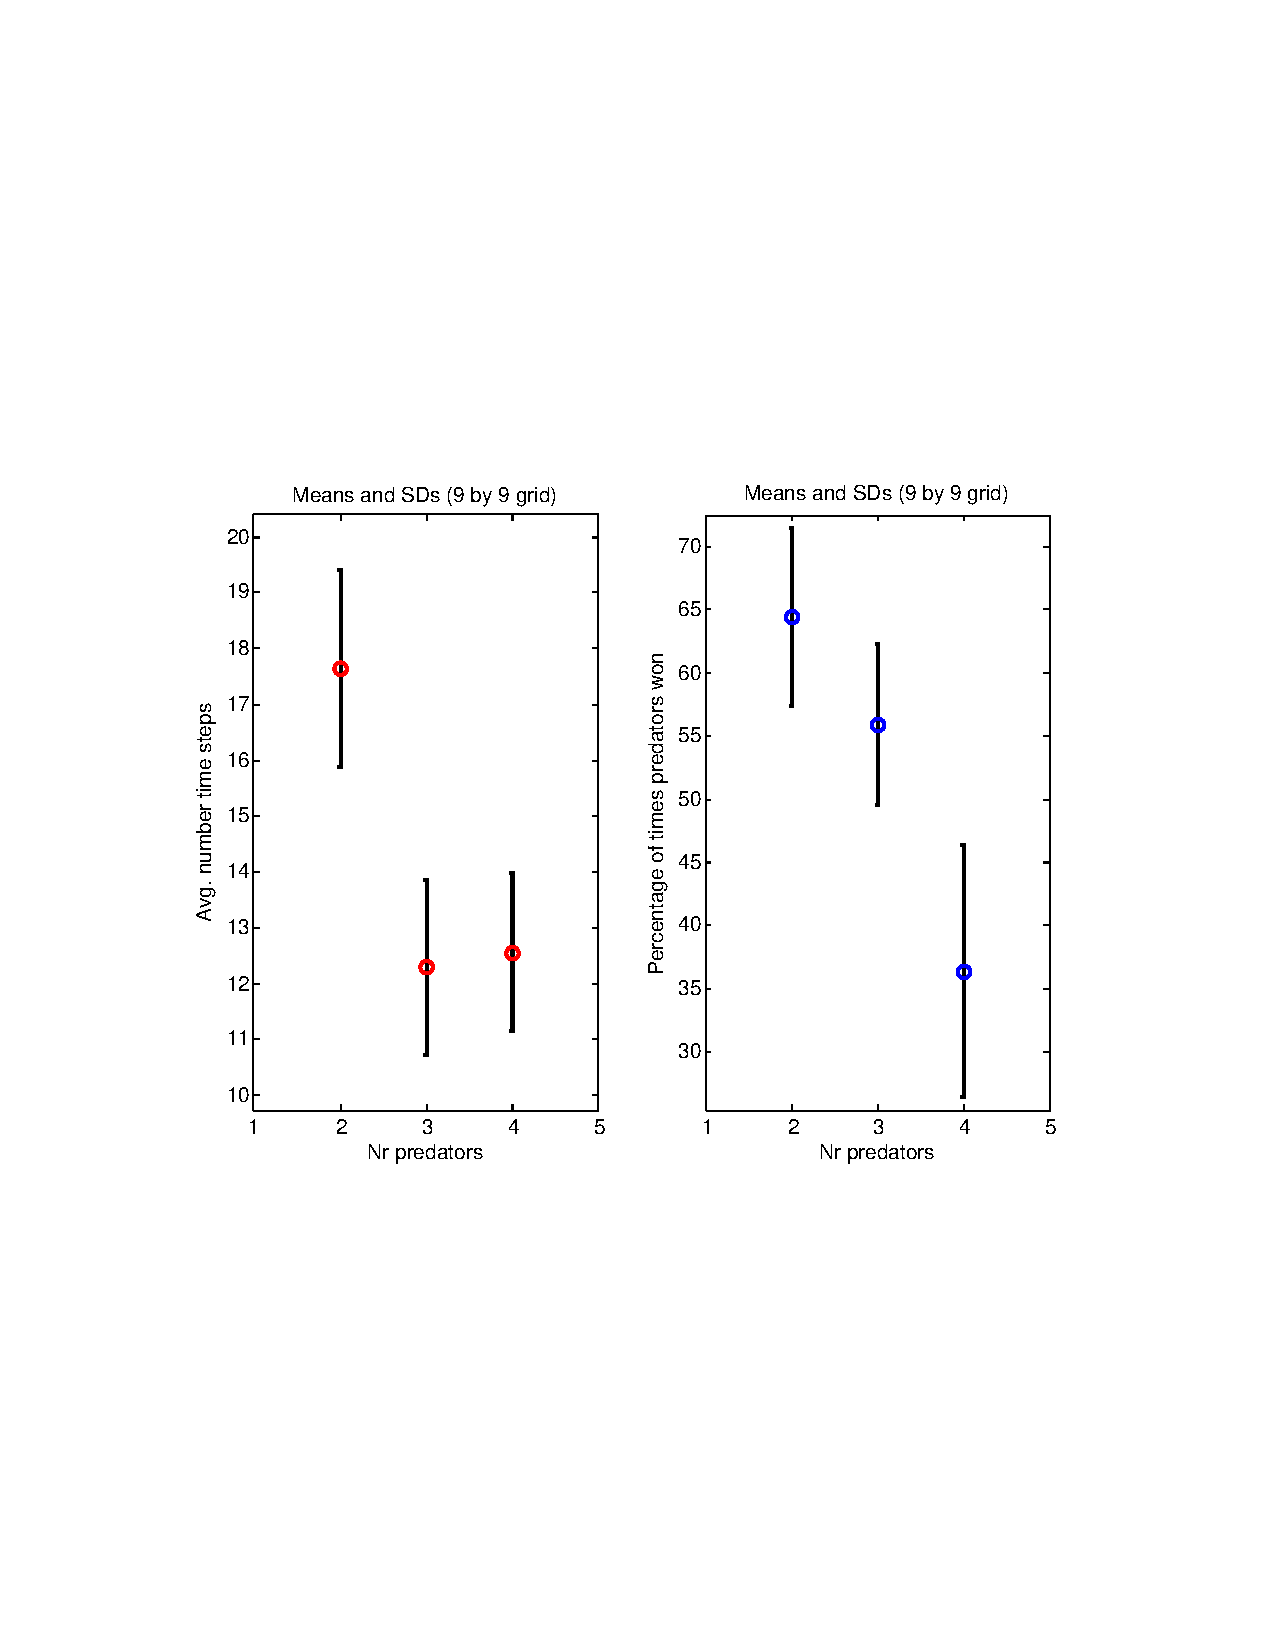
\includegraphics[bb = 0.6in 3in 7.9in 8.5in,clip,width=0.75\textwidth]{IQLgrid9by9ErrorBars.pdf} 
\caption{Means and SD's for performance measures for IQL, for 5000 episodes}
\label{fig:IQLmeansSds}
\end{figure}



We can see that in the case of four predators the percentage of times that the predators won an episode is the smallest. This is probably because of the higher chance of collision and more difficult coordination necessities. The variance for this measure for the case of four predators is also pretty high, also suggesting that a  ``common'' and more or less converged policy is not developed yet (insofar as a true common converged policy is possible under IQL). 

The case of there being three predators performs almost the same as the case of there being four predators on the average number of time steps  needed for termination of an episode. However for the case of there being three predators the episode endings are more often in the predators' favor. It seems, that three predators catch the prey less often than when there are two predators, but they do need less time steps for it.
 
On the other hand, the case of there being two predators performs surprisingly well on the percentage of times the predators won, but needs a lot of time steps for that.

\FloatBarrier

Now it would be interesting to see the performance over time and also if IQL actually converges for these cases, since IQL is not guaranteed to.
In Tables \ref{tab:percentage} and \ref{tab:timeSteps} we show the mean and variance again but now also the last value (i.e. at the $5000\mathrm{th}$ episode, run 200 times) for the corresponding  measure.

\begin{table}[hbt]
\centering
\begin{tabular}{lllll}
 Nr. predators  &  Variance& Mean & Last value   \\ 
\hline   
 2 & 50.109 & 64.482 & 62   \\ 
 3 & 41.104 & 55.941 & 62.5   \\ 
 4 & 99.92  & 36.331 & 60   \\  
\end{tabular} 
\caption{Percentage of times predators won (9 $\times$ 9 grid)}
\label{tab:percentage}
\end{table}

\begin{table}[hbt]
\centering
\begin{tabular}{lllll}
 Nr. predators  &  Variance& Mean & Last value   \\ 
\hline   
 2 &3.08 & 17.64 & 16.61   \\ 
 3 & 2.435 & 12.297 & 12.155   \\ 
 4 & 1.997  & 12.562 & 12.89   \\  
\end{tabular} 
\caption{Average number of time steps  (9 $\times$ 9 grid)}
\label{tab:timeSteps}
\end{table}

We can immediately see that the case of four predators seems to catch pretty well up for the measure of the percentage of times they won. Its mean value is 36.331 but its end value is 60. The case for two predators seems to have ``converged'' long before, with a mean close to its last value.

The variance of the case of four predators, for the measure of the percentage of times they won, is quite large.
This can mean the agents either learn very slow or because of large fluctuations in the distribution of ``skill'' over the prey and predators over time. In Figure \ref{fig:IQLpercentagePlot} we show a plot of the percentage of times the predators won for each predator number setting. We indeed see that in the setting of four predators the learning simply occurs slowly.


 In Figure \ref{fig:IQLpercentagePlot} we also see that the predator performance slowly goes down between the 500th and 2000th episode for the case of two predators. Apparently the predators learned to optimize their performance before the prey could, but then the prey learned their policy, and after that escapes more often. The predators apparently can't make a much better policy after that. For the settings of three and four predators, it seems the prey was the first to learn a (up until a certain time) good policy.
 
As for convergence, the average number of time steps used per episode seems to converge for all three settings, as can also be seen in Figure \ref{fig:IQLnrTimeSteps} (and Table \ref{tab:timeSteps}). The percentage of times the predators won, seems to converge for $5000$ episodes only for the settings of two and three predators. The value for four predators seems not stable yet, as can be seen in Figure \ref{fig:IQLpercentagePlot} (and Table \ref{tab:percentage}).



\begin{figure}[htb]
\centering
%bb = llx, lly, urx, and ury;
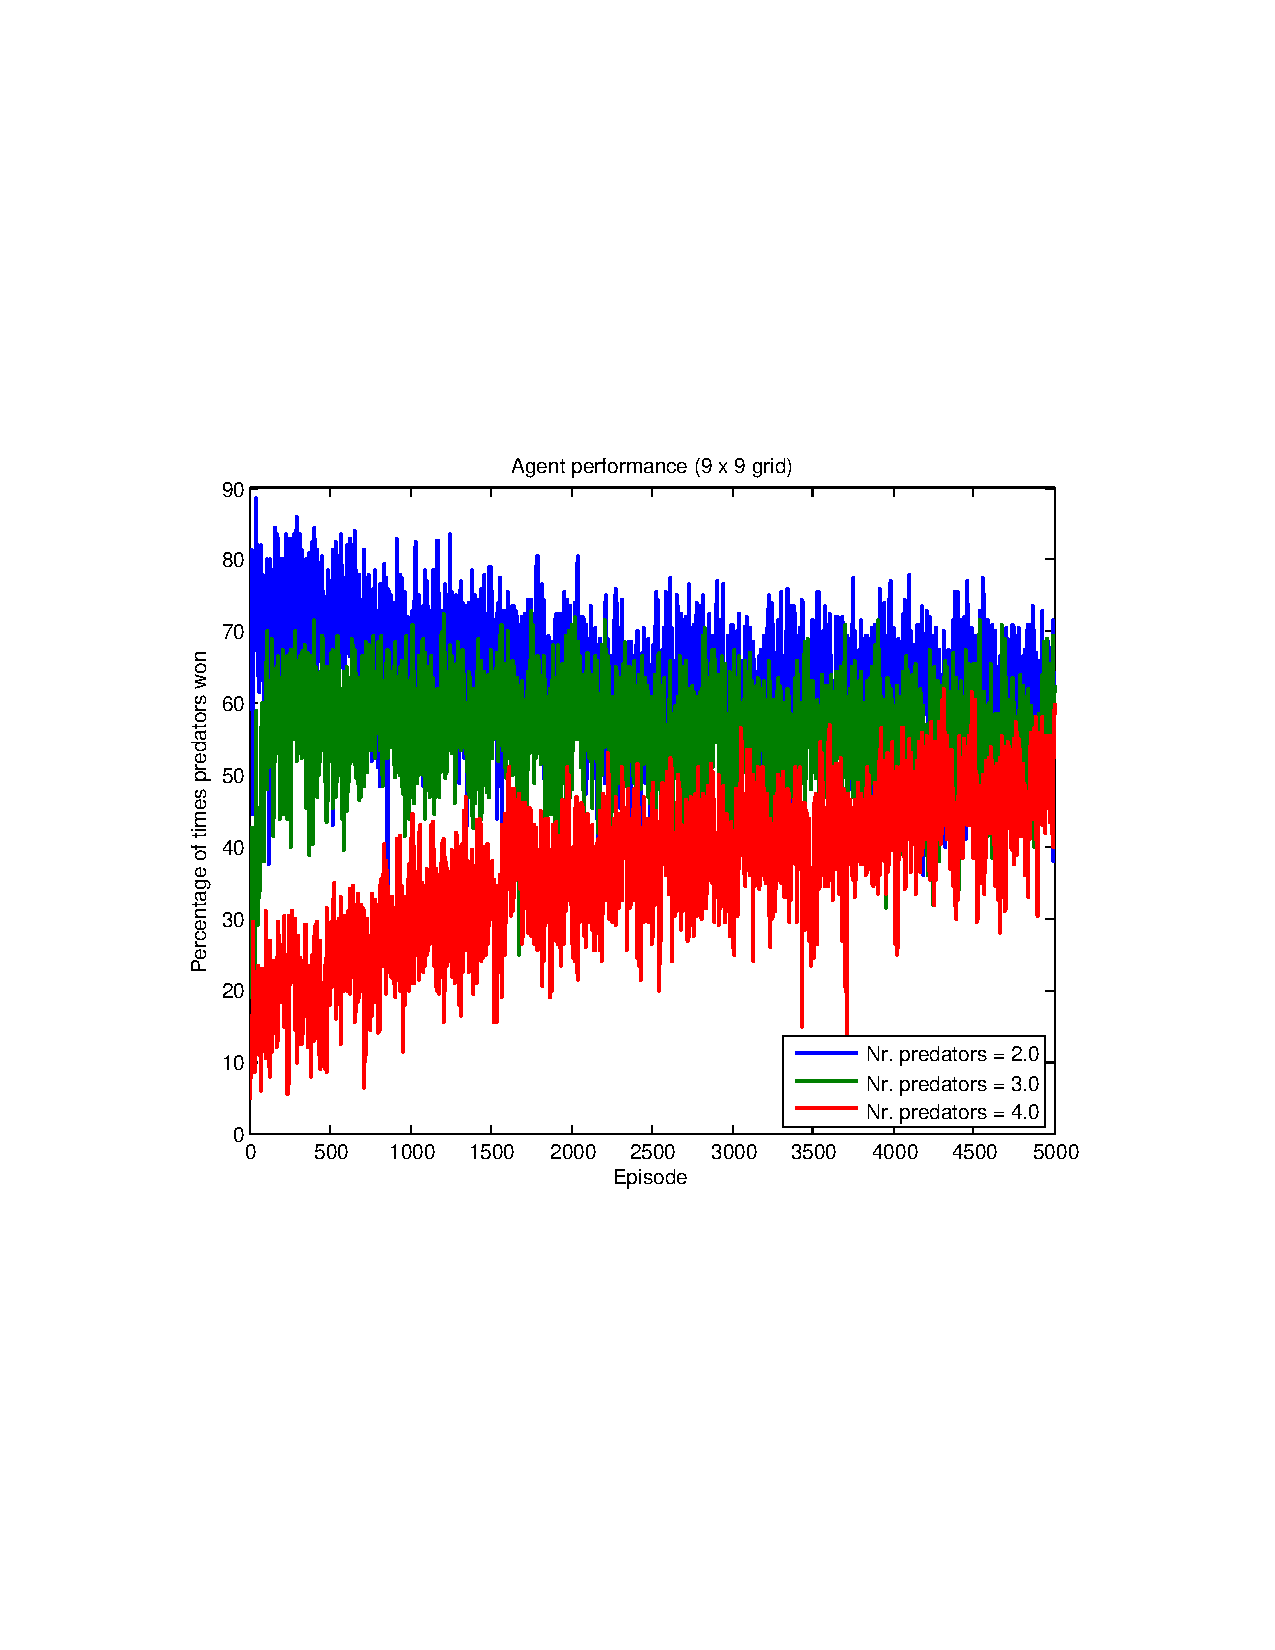
\includegraphics[bb = 0.6in 3in 7.9in 8in,clip,width=0.66\textwidth]
{IQLgrid9by9percentageWinning5000episodesavg200trials.pdf} 
\caption{Percentage of times the predators won for the three predator number settings}
\label{fig:IQLpercentagePlot}
\end{figure}
\begin{figure}[htb]
\centering
%bb = llx, lly, urx, and ury;
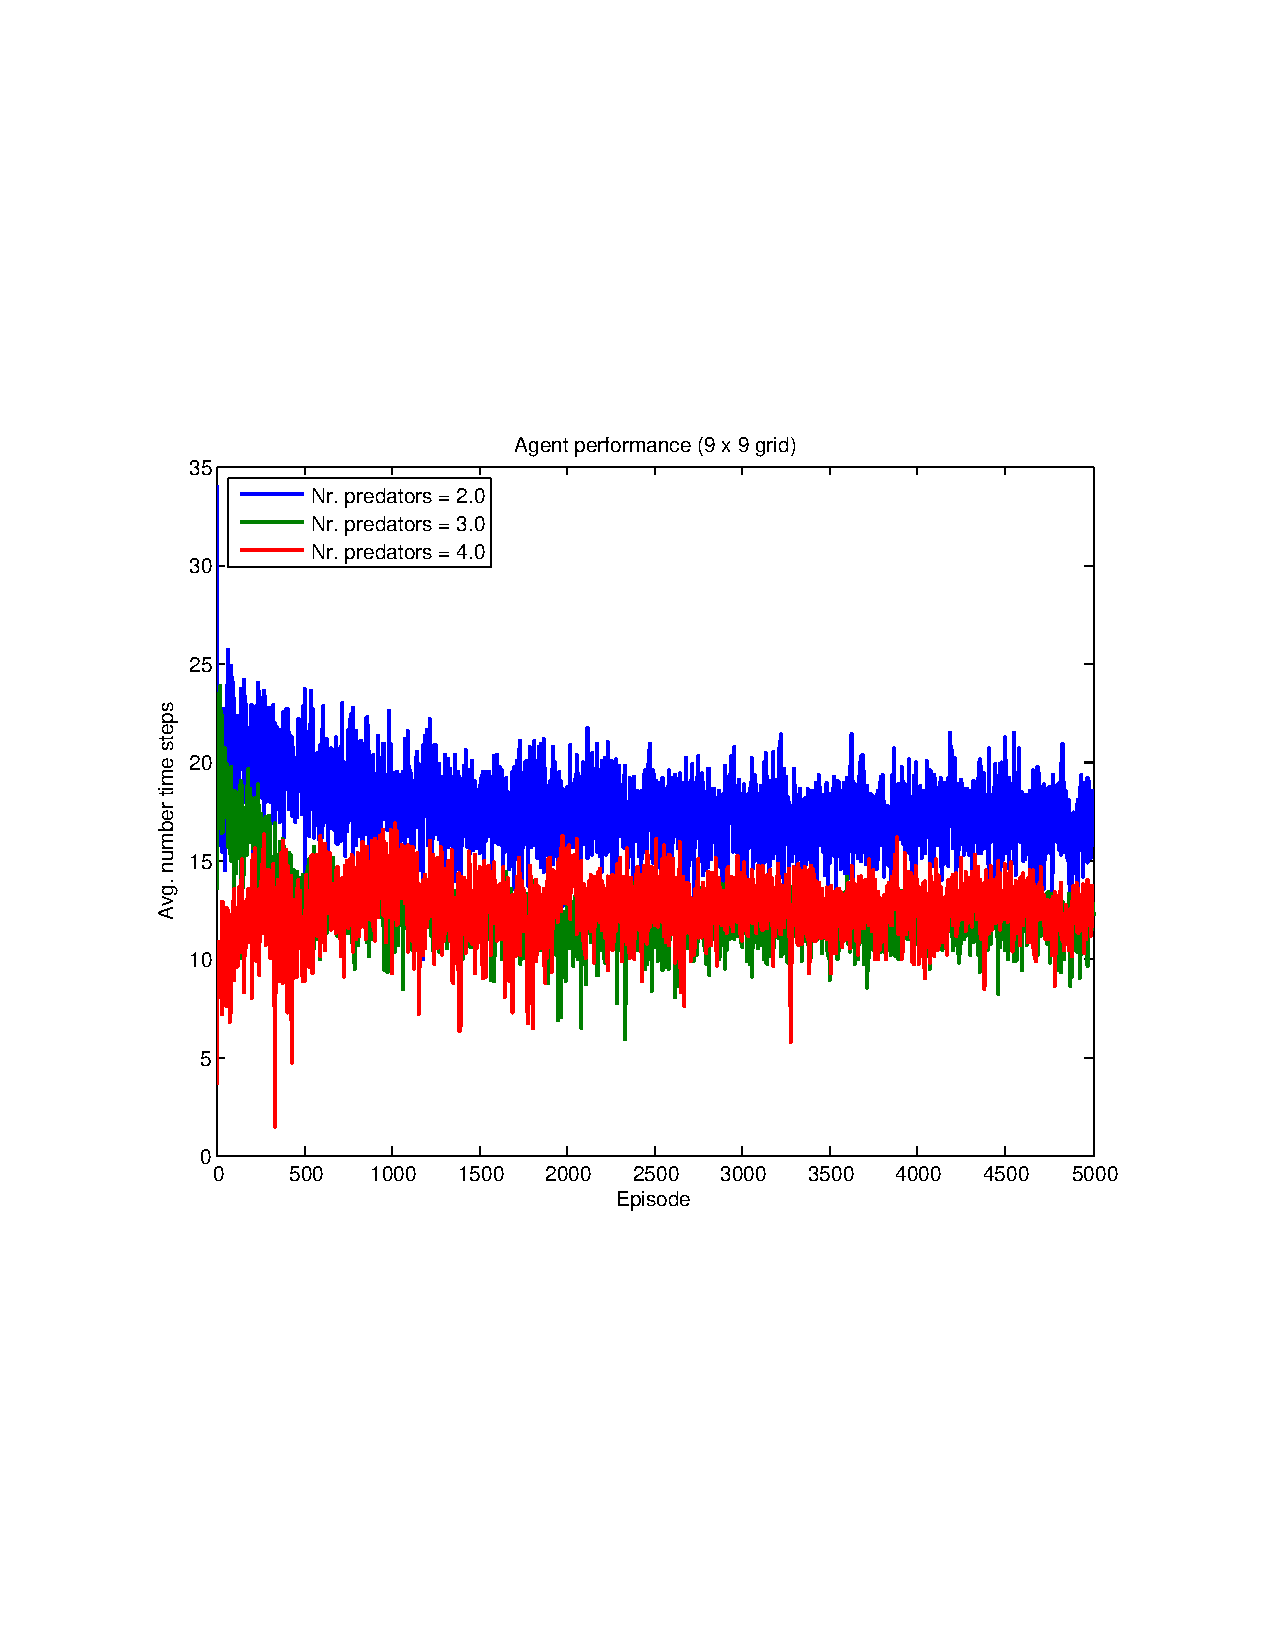
\includegraphics[bb = 0.6in 2.9in 7.9in 8.2in,clip,width=0.66\textwidth]
{IQLgrid9by9nrTimeSteps5000episodesavg200trials.pdf} 
\caption{Average nr. of time steps before an episode ending, for the three predator number settings}
\label{fig:IQLnrTimeSteps}
\end{figure}


\FloatBarrier
\clearpage
\subsubsection{Using an 11 $\times$ 11 grid}

The results for using a larger, $11 \times 11$ grid seem roughly similar to those in Section \ref{sec:IQLresults1} were we used a $9 \times 9$ grid. Compare Figure \ref{fig:IQLpercentagePlot2} with Figure \ref{fig:IQLpercentagePlot} and Figure \ref{fig:IQLnrTimeSteps2} with Figure \ref{fig:IQLnrTimeSteps}. The differences seem more pronounced for the first 1000 episodes. Also, the percentage of times that the predators won, is  higher for the case of three predators in the $11 \times 11$ setting, probably because of less collision issues.

\begin{figure}[hbt]
\centering
%bb = llx, lly, urx, and ury;
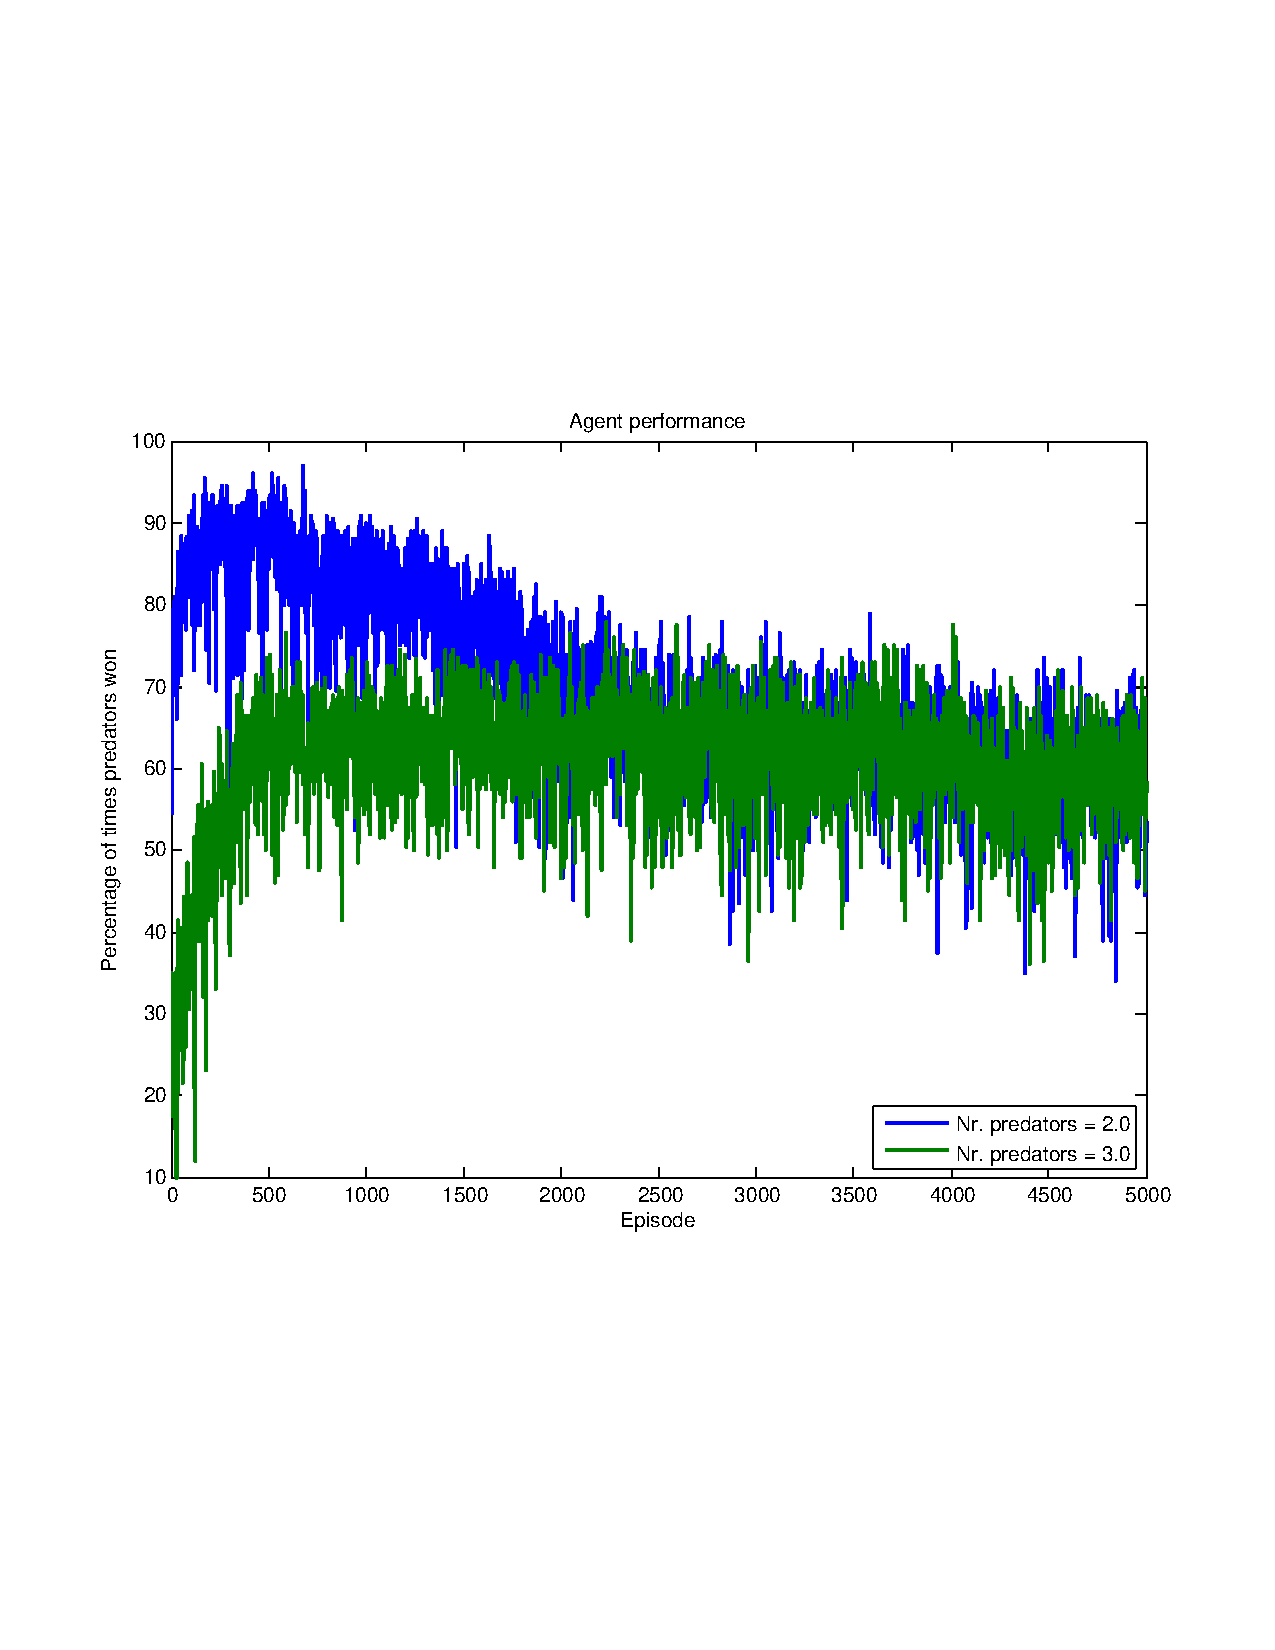
\includegraphics[bb = 0.6in 3in 7.9in 8.3in,clip,width=0.6\textwidth]
{IQLpercentageWinning5000episodesavg200trials.pdf} 
\caption{Percentage of times the predators won for the three predator number settings}
\label{fig:IQLpercentagePlot2}
\end{figure}
\begin{figure}[hbt]
\centering
%bb = llx, lly, urx, and ury;
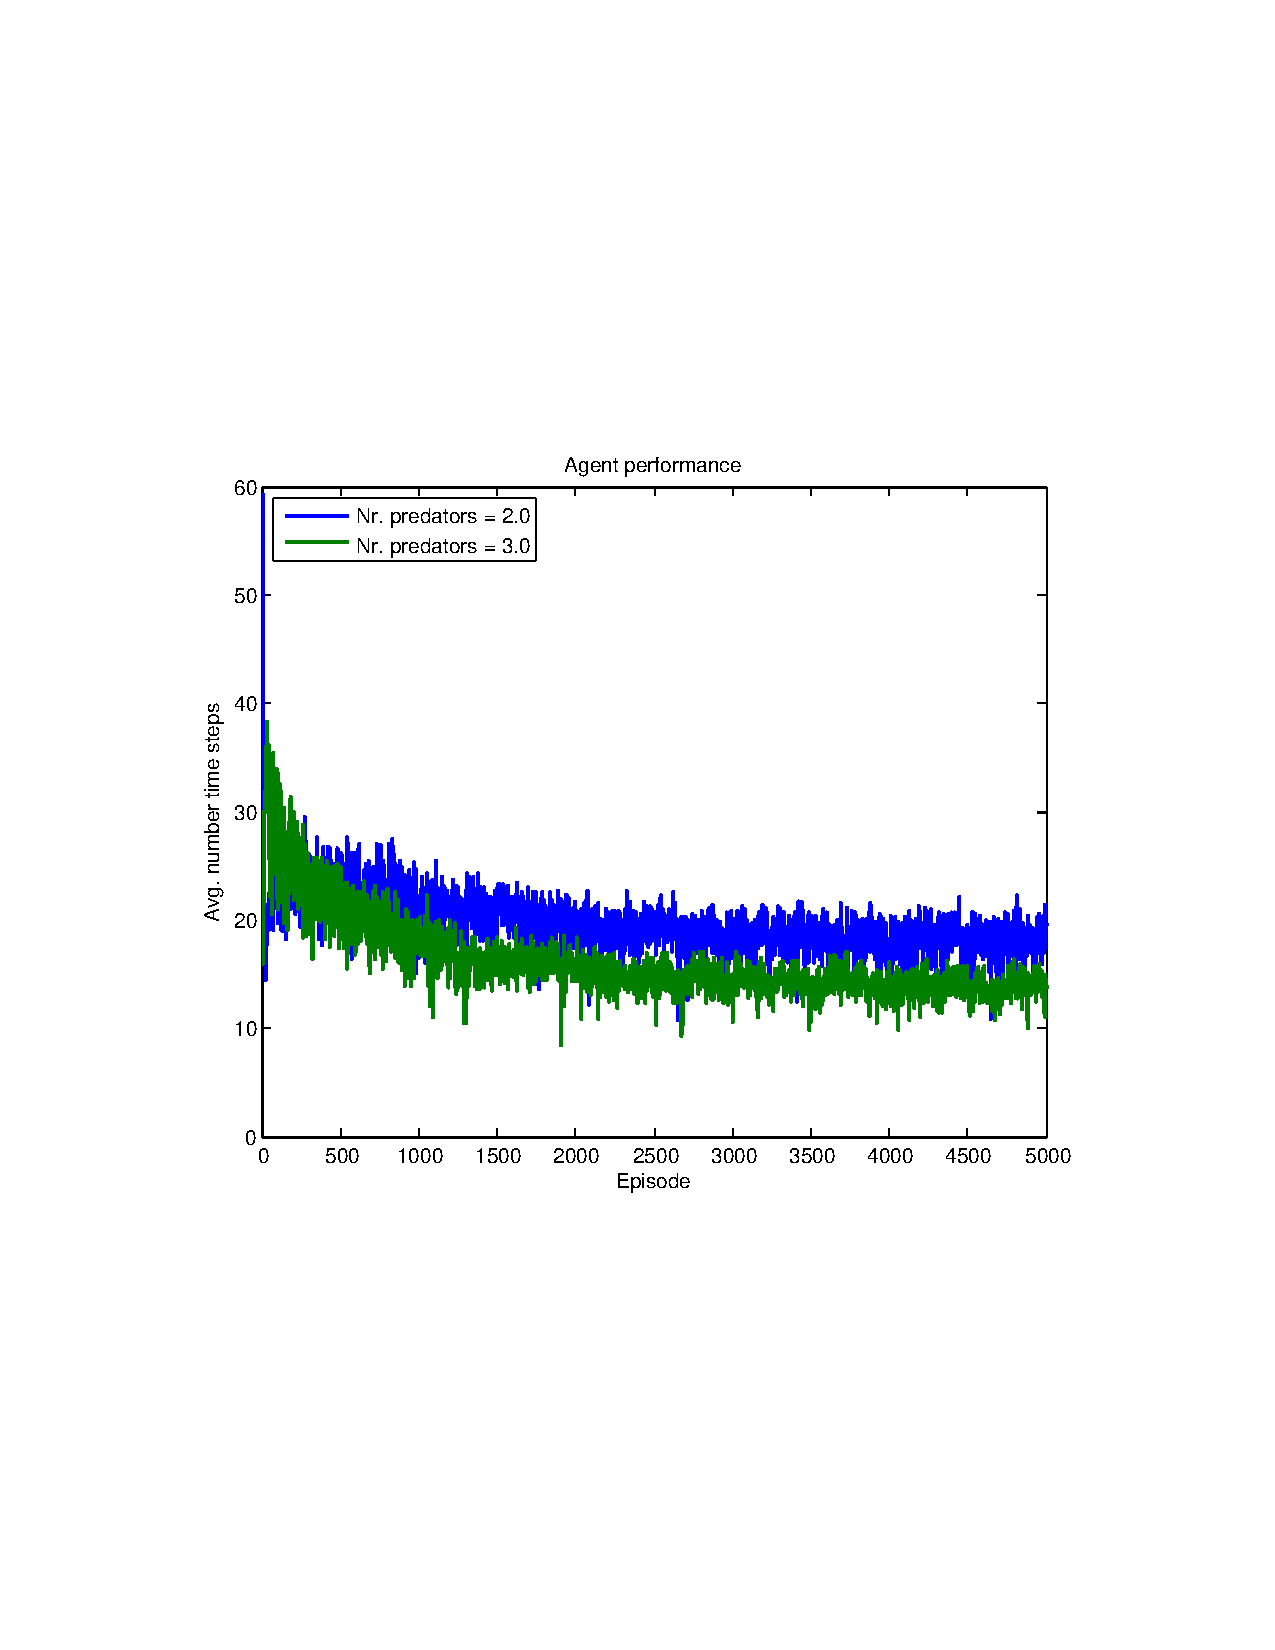
\includegraphics[bb = 0.6in 3in 7.9in 8in,clip,width=0.73\textwidth]{IQLnrTimeSteps5000episodesavg200trials.pdf} 
\caption{Average nr. of time steps before an episode ending, for the three predator number settings}
\label{fig:IQLnrTimeSteps2}
\end{figure}


\clearpage